%Lab template made by Joshua Milas for the EEEE labs

\def \labnum	{\#2}
\def \tonames   {Tyler Nicholson}
\def \disptitle	{MOSFET Characterization}
\def \datestart	{03-06-2015}
\def \dateend	{03-20-2015}

%Lab template made by Joshua Milas for the EEEE labs
%Modified highly by Chris Culpepper



\documentclass[12pt]{article}	%12 point font

\usepackage{amsmath}	%Provides features and environments to help writing math equations, such as the align environment
\usepackage{graphicx}	%provides some extra features for including graphics. Optional
\usepackage[margin=0.8in]{geometry}	%Set the margins of the paper
\usepackage{float}	%Provides the [H] for hard setting things. It means "Put this exactly her
\usepackage{circuitikz}	%Used for circuit drawing
\usepackage[export]{adjustbox}	%Used for alligning the RIT image to the right
\usepackage[outdir=./]{epstopdf}	%Used to include .eps vector images
\usepackage{indentfirst} %So the first line of a section is indented
\usepackage{titlesec} %To reduce the space after section titles
\usepackage{caption} %For caption junk
\usepackage{siunitx} % Formats the units and values
\usepackage{pgfplotstable} % Generates table from .csv
\usepackage{commath} %Used for math functions

\usepackage{datatool} %For the importation of CSVs to tables
\usepackage{colortbl} %So every other row of the table con be gray
\usepackage{fancyhdr} %For header and footer functionalithy
\usepackage{lastpage} %To get the last page num for the footer.
\usepackage{xcolor} %For different colors. 

\definecolor{light-gray}{gray}{0.85} %The gray color used for every other row in the table 

%To get numbers into Engineering notation, use \num{thhe number here} 
\sisetup{exponent-product = \times ,round-mode = figures,%
	  round-precision = 5, scientific-notation = engineering}

%These are the caption declarations for equations and tables. 
\DeclareCaptionType{equationCaption}[][List of equations]
\DeclareCaptionType{tableCaption}[][List of Tables]
\captionsetup[equationCaption]{name=Equation}%{labelformat=Equation}
\captionsetup[tableCaption]{name=Table}%{labelformat=Equation}

%For the pictures, i think
\epstopdfsetup{outdir=./}

%To move the section titles to match the format. 
\titlespacing\section{0pt}{5pt}{-2em}


\newcommand{\tab}{\hspace*{1.5em}}	%Tab command
\newcommand{\newsection}[1]{\setlength{ 	%Make a section
	\section*{#1}
	\leftskip}{0em}
	\vspace{5ex}
	%\setlength{\leftskip}{1em}
}
%This pretty prints an equation. 
%1st arg: The label to be used for reference 
%2nd arg: The equation. Use Math Mode. 
%3rd arg: The caption text. 
\newcommand{\eq}[3]{
	\begin{equationCaption}[H]
		\begin{equation}
			#2
			\label{#1}
		\end{equation}
		\caption{#3}
	\end{equationCaption}}
%Adds an image, captions and labels. 
%1: Optional arguments to \includegraphics. Use to set image params. 
%2: The filename
%3: The caption
%4: The label for referential purposes. 
\newcommand{\nimg}[4][]{
	\begin{figure}[H]
		\centering
		\includegraphics[#1]{#2}
		\caption{#3}
		\label{#4}
	\end{figure}
}
%Adds a table by CSV. Adds caption, label. 
%1 The label
%2 The filename
%3 The caption
\newcommand{\ntab}[3]{
	\DTLloaddb{#1}{#2}
	\arrayrulecolor{black}
	\begin{table}[H]
		\centering
% Work out the column alignments.
		\def\colalign{}%
		\dtlforeachkey(\theKey,\theCol,\theType,\theHead)\in{#1}\do
		{\edef\colalign{\colalign l}}%
% Begin the tabular environment.
		\edef\dobegintabular{\noexpand\begin{tabular}{\colalign}}%
			\dobegintabular
			%\toprule

% Do the header row.
			\gdef\doamp{\gdef\doamp{&}}%
			\renewcommand{\dtlbeforecols}{|}
			\renewcommand{\dtlaftercols}{|}
			\dtlforeachkey(\theKey,\theCol,\theType,\theHead)\in{#1}\do
			{\doamp\bfseries \theHead}%
% Iterate through the data.
			\\%\midrule
			\\[-5ex]
			\DTLforeach{#1}{}{%
				\\\gdef\doamp{\gdef\doamp{&}}%
				\renewcommand{\dtlbeforecols}{a}
				\renewcommand{\dtlaftercols}{a}
				\renewcommand{\dtlbetweencols}{a}
				\\[-3ex]\DTLifoddrow{\rowcolor{light-gray}}{\rowcolor{white}}%

				\DTLforeachkeyinrow{\thisValue}{
					\doamp 
					\DTLifeq{\dtlcol}{1}{
						\thisValue
					}{
						\num{\thisValue}}
					}}%
						%\\\bottomrule
					\end{tabular}
					\caption{#3}
					\label{#1}
				\end{table}
			}
\begin{document}
%\maketitle
\pagestyle{fancy} %Sets up the page to fancy for the header. 
\fancyhf{} % sets both header and footer to nothing
\renewcommand{\headrulewidth}{0pt} %Used to remove the spacing in a header.
% your new footer definitions here
\renewcommand{\headsep}{0pt} %Removes extra headerspacing
\lfoot{EEEE381 Tech Memo Lab \labnum} %The left part of the footer
\cfoot{\dateend} %The due date
\rfoot{\thepage\ of \pageref{LastPage}} %The right footer

 %Starts the RIT logo
\begin{flushright}
\begin{figure}[H]
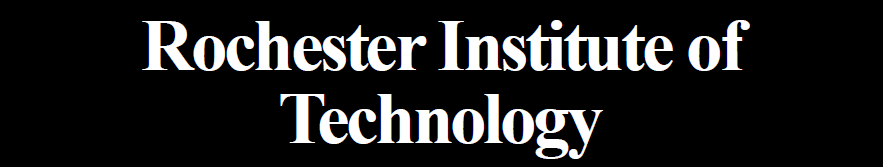
\includegraphics[height=9ex,right]{../title.png}
\end{figure}
\end{flushright}
\noindent
\\[-3em] %Removes extra space. Jankily. 
 %Starts the title
\huge
\textbf{EEEE 381 - Electronics I \\[1ex] Techical Memorandum}\\
\normalsize

 %This is the to/from garbage. Should probably make the name and section numbers variable
\noindent
\begin{tabular}{ll}
\textbf{From:} &Christopher Culpepper (Computer Engineering)\\
\textbf{Partner:} &N/A\\
\textbf{To:} &To: \tonames\ | Section L3\\
\textbf{Date:} &Performed: \datestart; Due: \dateend\\
\textbf{Subject:} &Lab \labnum: \disptitle
\end{tabular}

\noindent
\rule{\textwidth}{.1pt}
%\\[-2em]





\hyphenation{MOSFET} %Makes MOSFET not hyphenated


\newsection{Abstract}
The purpose of this exercise was to gain increased understanding of the Metal Oxide Semiconductor Field Effect Transistor (MOSFET) through calculations and experimentation. 
During the pre-exercise. graphs were made predicting various voltage and current relationships for the MOSFET and from these graphs, methods of calculating various MOSFET parameters were derived. 
During the experiment, measurements were taken of input voltages and the resulting current for multiple MOSFET circuits with multiple changing parameters. 
From these measurements, MOSFET values were calculated and found to be close to the values from the datasheet. 


\newsection{Theory}
A MOSFET is said to be operating in saturation if the voltage between the source and the drain is greater than the difference between the gate voltage and the voltage threshold, or $V_{DS} \geq (V_{GS}-V_t)$ for an NMOS transistor. The condition for a PMOSFET is similar, except the fact that $V_{GS}$, $V_{DS}$ and $V_t$ are negative. 
While in saturation, the current can be simply modeled using the equation shown in equation \ref{eq:nmosSatCurr}.
\eq{eq:nmosSatCurr}{i_D= \frac{1}{2}* k'_n \frac{W}{L}(V_{GS}-V_t)^2(1+\lambda(V_{DS}-V_{DSsat}))}{NMOSFET Saturated Current Equation}
For a small error, the channel length modulation term, $(1+\lambda(V_{DS}-V_{DSsat}))$, can be omitted. The result of this is shown in equation \ref{eq:nmosSatCurrNoCLM}. 
\eq{eq:nmosSatCurrNoCLM}{
	i_D= \frac{1}{2}* k'_n \frac{W}{L}(V_{GS}-V_t)^2}
	{NMOSFET Saturated Current Equation Without Channel Length Modulation}
Note that the eqation in \ref{eq:nmosSatCurrNoCLM} can be applied to a PMOS device by negating $V_{GS}$ and $V_t$. All of the following equations will be for NMOS devices and can be applied to PMOS devices by negating terms. 
By taking the square root of each side in equation \ref{eq:nmosSatCurrNoCLM}, the parameters $V_t$ and $k`_n \frac{W}{L}$ can be extracted from the slope and the y-intercept. 

The equation used to calculate $V_t$ and $k`_n \frac{W}{L}$ from a trendline of $\sqrt{i_D}$ Vs. $V_{DS}$ is shown in equation \ref{eq:sqrtIdVsVDS}. 
\eq{eq:sqrtIdVsVDS}{
	\sqrt{i_D}= \sqrt{\frac{1}{2}* k'_n \frac{W}{L}}*V_{GS}-V_t*\sqrt{\frac{1}{2}* k'_n \frac{W}{L}}}
	{Equation to Calculate $V_t$ and $k`_n \frac{W}{L}$}

%Part 6 Calculations:
When voltage is applied between the body and the source, the threshold voltage, $V_t$ changes as shown in equation \ref{eq:part6Init}.

\eq{eq:part6Init}{
	V_t=V_{t0} + \gamma ( \sqrt { 2\phi_f+V_{SB}} - \sqrt{2\phi_f})}
	{Threshold Voltage Calculation Equation}

% Part 7. 

$\gamma$, as shown in equation \ref{eq:part6Init}, is known as the body-effect parameter. $\phi_f$ is a physical parameter of the MOSFET and is typically in the range of 0.3 to 0.4 volts. 
$\gamma$ can be calculated by applying equation \ref{eq:part7}, where q is the charge of the carrier (Electron for NMOSFET and Hole for PMOSFET), $\epsilon_s$ is the permeability of silicon, $N_{sub}$ is the doping concentration and $C_{ox}$ is the oxide permittivity.  

\eq{eq:part7}{
	\gamma = \frac { \sqrt{ 2 q \epsilon_s N_{sub } }}{C_{ox}} 
	}{$\gamma$ Calculation Equation}

When $\gamma$ is known, $N_{sub}$ can be calculated through simple rearrangements of equation \ref{eq:part7}. The equation showing this is displayed in equation \ref{eq:part7Nsub}. 

\eq{eq:part7Nsub}{
	N_{sub}=\frac{(\gamma C_{ox} )^2}{2 q \epsilon_s}}
	{$N_{sub}$ Calculation Equation}
The parameter $C_{ox}$ can be calculated using equation \ref{eq:coxEq}, where $\epsilon_0$ is the permittivity of the oxide, 3.4531E-11 and $t_{ox}$ is the thickness of the oxide. 
\eq{eq:coxEq}{C_{ox}= \frac{\epsilon_0}{t_{ox}}}{Equation for the Calculation of $C_{ox}$}


%Part 7 part 2

$N_{sub}$ can also be calculated using equation \ref{eq:part72init}. To calculate $N_{sub}$ in this way, first the carrier mobilities, $\mu_n$ and $\mu_p$ must be calculated. $\mu$ can be calculated from $k`_n \frac{W}{L}$, $\frac{W}{L}$ and $C_{ox}$ through the equation in equation \ref{eq:mucalc}, which was derived from the MOSFET current equation. 
\eq{eq:part72init}{
	\mu = \mu_{min} + \frac { \mu_{max} - \mu_{min}}{1 + ( \frac{N_{sub}}{N_{ref}} ) ^ a}}
	{Equation Relating $\mu$ and $N_{sub}$}

\eq{eq:mucalc}{
	\mu_n = \frac{2k`_n \frac{W}{L}}{\frac{W}{L}}}
	{Equation for the Calculation of $\mu$}
Equation \ref{eq:part72init} can be rewritten to better facilitate the calculation of $N_{sub}$. This is shown in equation \ref{eq:part72fin}. 
\eq{eq:part72fin}{
	N_{sub}=N_{ref}* \sqrt[a]{\frac{\mu_{max} - \mu_{min}}{\mu-\mu_{min}}-1}}
	{Calculation of $N_{sub}$}
Another important parameter of the MOSFET is the channel length modulation parameter $\gamma$. This factor affects the slope of the current increase while the MOSFET is in saturation. Where this slope intersects the horizontal is the early voltage, $V_A$. The inverse of $V_A$ is $\gamma$. Using $\gamma$ to supplement the simplified current equation leads to a more accurate calculation. 
% Bout time. Part 8 part 2......
The early voltage can also be calculated using terms given in the MOSFET datasheet, $I_D$ and $G_{DS}$, the drain current and output transconductance parameters. The equation to calculate $V_A$ is shown in equation \ref{eq:part82}.
\eq{eq:part82}{
	V_A = \frac{I_{DS}}{G_{DS}}
	}{Calculation of $V_A$}

\newsection{Results}
The results for part 1 are shown in figure \ref{fig:p1nmos} and \ref{fig:p2pmos}.
\nimg{fig:p1nmos}{part1.png}{$I_D$ Vs $V_{DS}$ NMOS}
\nimg{fig:p2pmos}{part2.png}{$I_D$ Vs $V_{SD}$ PMOS}


From the data collected for part one of the exercise, $V_t$ and the transconductance parameter,$k=k'* \frac{W}{L}$, can be calculated from equation \ref{eq:sqrtIdVsVDS} by plotting $\sqrt{I_D}$ Vs. $V_{GS}=V_{DS}$ and calculating a linear trendline.

The data showing $\sqrt{I_D}$ Vs. $V_{GS}=V_{DS}$ is shown in the appendix in table \ref{tbl:part5NMOS} for the NMOS device and in table \ref{tbl:part5PMOS} for the PMOS device. 
Plots of these data, along with the computed trendlines are shown in figures \ref{fig:part5NMOS} and \ref{fig:part5PMOS} for the NMOS and PMOS devices. 
Note that when the voltage applied to the body increases, the required voltage applied to the drain also increases to bring the device into the linear region. To ensure the trendline was accurate, some of the data at low drain voltages was omitted from the graph. This complete data is shown in the tables in the appendix. 

Also note that because the PMOSFET measurements were taken negatively with respect to the NMOSFET, the value for $V_t$ is positive. If the measurements were taken the same way as with the NMOSFET, the value for $V_t$ would have been negative. The sign for the threshold voltage does not matter as long as it is taken into account. 

\nimg[]{fig:part5NMOS}{part5NMOS.png}{$\sqrt{I_D}$ Vs. $V_{GS}=V_{DS}$ For NMOSFET}
\nimg[]{fig:part5PMOS}{part5PMOS.png}{$\sqrt{I_D}$ Vs. $V_{SG}=V_{SD}$ For PMOSFET}

From the trendlines, $V_t$ and $k$ were calculated. The results of this for differing values of $\abs{V_{SB}}$ are shown in table \ref{tbl:part5FinRes}. Only the values of k for the $|V_{SB}|$ = 0 are needed, but all are shown. 
\ntab{tbl:part5FinRes}{part5FinRes.csv}{Calculated values of $V_t$ and $k$}
Plotting the calculated values of $V_t$ against $\sqrt{2\phi_f+\abs{V_{SB}}}+\sqrt{2\phi_f}$ allows for the calculation of the body effect parameter, $\gamma$. Initially, $2\phi_f$ can be approximated to be 0.6V. Using this, $\gamma$ can be calculated. The data for this plot is shown in table \ref{tbl:part6} and the plots of these data are shown in figure \ref{fig:part6Plot}. 
\nimg[width=6in]{fig:part6Plot}{part6.png}{$V_t$ Vs.  $\sqrt{2\phi_f+|V_{SB}|}+\sqrt{2\phi_f}$ for NMOSFET and PMOSFET}
The calculated values for $\gamma$ are shown in table \ref{tbl:part6FinRes}. 

\ntab{tbl:part6FinRes}{part6FinRes.csv}{Calculated values for $\gamma$ for the NMOSFET and PMOSFET}
%Begin shit for part7. 2 left...........

By applying equation \ref{eq:part7Nsub}, the values calculated for $\gamma$, $C_{ox}$, and $\epsilon_s$, the permittivity of silicon, $1.05*10^{-10}$, the values for $N_{sub}$ can be found. These values are shown in table \ref{tbl:part7Res}. 
\ntab{tbl:part7Res}{part7.csv}{Calculated Values for $N_{sub}$}

%Last part of 7...
Calculating $N_{SUB}$ through equation \ref{eq:part72fin}, leads to the results shown in figure \ref{tbl:part72fin}.
\ntab{tbl:part72fin}{part72fin.csv}{Calculation of $N_{SUB}$ through $\mu$}
% fuck 7, go to 8
By plotting $I_D$ against $|V_{DS}|$ for a transistor with its body tied to the source and a constant $|V_{GS}| = 2.5V$, the channel length parameters, $\lambda_n$ and $\lambda_p$ can be found from the horizontal-intercepts by way of finding the early voltage, $V_A$.
The plot showing $I_D$ Vs. $|V_{DS}|$ is shown in figure \ref{fig:part8plot} and the data for the plot in table \ref{tbl:part8}. 
\nimg[width=6in]{fig:part8}{part8.png}{$I_D$ Vs. $|V_{DS}|$}
Once $V_A$ was found, its inverse was used to calculate the $\lambda$ parameter. This data, as well as the manufacturer specified values are shown in table \ref{tbl:part8finnmos} for the NMOSFET and in table \ref{tbl:part8finpmos} for the PMOSFET. 
\ntab{tbl:part8finnmos}{part8finnmos.csv}{Measured and Calculated $\lambda$ and $V_A$ for NMOSFET}
\ntab{tbl:part8finpmos}{part8finpmos.csv}{Measured and Calculated $\lambda$ and $V_A$ for PMOSFET}
\newsection{Conclusion}
Overall the exercise was a success. The MOSFETs parameters were measured and found to be close to parameters from the datasheet, or at least were not off by a large factor. 
Values may have been off due to experimental error or measurement difficulties. When measuring small currents, the multimeter does not have enough accuracy. In addition to this, despite trying to keep the voltage source at precisely the required voltage, the built in meter was slightly off. \\
Trouble was had when calculating results from the measured data as the equations derived in prelab were incorrect as well as not available. Despite this, new equations were derived and the results shown were calculated. 




\newsection{Appendix}
\ntab{tbl:part5NMOS}{part5NMOS.csv}{$\sqrt{I_D}$ Vs. $V_{GS}=V_{DS}$}
\ntab{tbl:part5PMOS}{part5PMOS.csv}{$\sqrt{I_D}$ Vs. $V_{SG}=V_{SD}$}
%\ntab{tbl:part6}{part6.csv}{test}
\ntab{tbl:part6}{part6.csv}{$V_t$ Vs.  $\sqrt{2\phi_f+|V_{SB}|}+\sqrt{2\phi_f}$}
\ntab{tbl:part8}{part8.csv}{$I_D$ Vs. $|V_{DS}|$}
\end{document}
